\section{逆热问题}
\label{sec:heat-inverse}

设想测得了棒在时刻$T$的温度，想知道时刻$0$的温度。这称为\term{逆热问题}（backward heat problem）。方程本身可逆吗？正向问题适定，反向问题是否同样？

\paragraph{高频被放大}
在$(0,1)$上取零边值，$u(\cdot,T)$的坐标是$y_k=\mathrm{e}^{-\lambda_kT}c_k$。形式上，初值的坐标由$c_k=\mathrm{e}^{\lambda_kT}y_k$恢复，这一步把每个坐标放大$\mathrm{e}^{\lambda_kT}$倍。$T=0.05$时，
\[
 \mathrm{e}^{\lambda_1T}\approx1.64,\quad \mathrm{e}^{\lambda_3T}\approx84.9,\quad \mathrm{e}^{\lambda_5T}\approx2.3\times10^{5},\quad \mathrm{e}^{\lambda_7T}\approx3.2\times10^{10} .
\]
测量总有误差。正向传播把高频压没了，反向传播要把它放大回来，噪声也跟着放大。

图~\ref{fig:heat-inverse-amplify}(b)、(c)显示了问题的另一面：两个明显不同的初值，到$T=0.05$时几乎无法区分。差的部分是$0.12\sin(11\pi x)$，放大因子使它在终态只剩约$10^{-27}$，任何测量都看不出来。

\begin{BookInlineFigure}
  \centering
  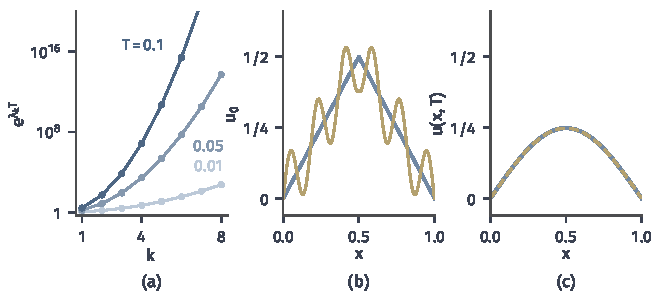
\includegraphics[width=112mm]{figures/06-differential-equations/02-partial-differential-equations/matplotlib/heat-inverse-amplify/figure.pdf}
  \caption{反向恢复的困难。(a)放大因子$\mathrm{e}^{\lambda_kT}$，$T=0.01,0.05,0.1$（蓝色由浅到深），纵轴为对数。(b)三角形初值（蓝）及加上$0.12\sin(11\pi x)$的初值（黄）。(c)二者在$T=0.05$时的解，两条曲线重合。}
  \label{fig:heat-inverse-amplify}
\end{BookInlineFigure}

\paragraph{不适定性}
正向映射是单射，所以终态确实决定初态。可是Hadamard的三条要求中，存在性和连续依赖都失败，这就是\term{不适定问题}（ill-posed problem）的情形。

\begin{theorem}[逆热问题的不适定性]
\label{thm:heat-inverse-illposed}
设$S(T):L^2(0,1)\to L^2(0,1)$是零Dirichlet条件的解算子，$T>0$。
\begin{enumerate}
 \item $S(T)$是单射；$y=\sum_ky_ke_k$属于其值域，当且仅当
 \begin{equation}
  \sum_k\mathrm{e}^{2\lambda_kT}y_k^2<\infty .
  \label{eq:heat-inverse-range}
 \end{equation}
 \item 逆映射不连续：存在$\lVert\eta_n\rVert_2\to0$的扰动，使$\lVert S(T)^{-1}\eta_n\rVert_2\to\infty$。
\end{enumerate}
\end{theorem}

\begin{proof}
(1)若$S(T)u_0=0$，则$\mathrm{e}^{-\lambda_kT}c_k=0$，所以全部$c_k=0$。$y=S(T)u_0$当且仅当$c_k=\mathrm{e}^{\lambda_kT}y_k$平方可和，这就是式~\eqref{eq:heat-inverse-range}。

(2)取$\eta_n=\mathrm{e}^{-\lambda_nT/2}e_n$。它的范数$\mathrm{e}^{-\lambda_nT/2}\to0$。而
\[
 S(T)^{-1}\eta_n=\mathrm{e}^{\lambda_nT/2}e_n,
\]
范数趋于无穷。
\end{proof}

式~\eqref{eq:heat-inverse-range}说，只有极其光滑的函数才是可能的终态。一个带噪声的观测几乎一定不满足它，形式公式的级数发散。

\paragraph{中间时刻的稳定性}
恢复$t=0$是不可能稳定的，但恢复稍早的时刻$0<t<T$好得多，只要预先知道初值有界。由Hölder不等式，取指数$T/(T-t)$与$T/t$，把$c_k^2\mathrm{e}^{-2\lambda_kt}$写成$(c_k^2)^{1-t/T}(c_k^2\mathrm{e}^{-2\lambda_kT})^{t/T}$，
\begin{equation}
 \lVert u(\cdot,t)\rVert_2\leq\lVert u_0\rVert_2^{\,1-t/T}\,\lVert u(\cdot,T)\rVert_2^{\,t/T} .
 \label{eq:heat-log-convexity}
\end{equation}
如果$\lVert u_0\rVert_2\leq R$，两个候选解的差也满足这个不等式，所以观测误差$\delta$在时刻$t$产生至多$(2R)^{1-t/T}\delta^{t/T}$的误差。这个指数$t/T$随$t\to0$退化为零，反映出$t=0$处失去稳定性。

\paragraph{用截断恢复}
放弃高频，只恢复可靠的部分。设观测$y=S(T)u_0+\eta$，$\lVert\eta\rVert_2\leq\delta$。截断重建是
\begin{equation}
 u^{N}=\sum_{k\leq N}\mathrm{e}^{\lambda_kT}\langle y,e_k\rangle\,e_k .
 \label{eq:heat-truncated}
\end{equation}

\begin{theorem}[截断重建的误差]
\label{thm:heat-truncation}
若$u_0\in H^1_0(0,1)$，$\lVert u_0'\rVert_2\leq R$，则
\begin{equation}
 \lVert u^{N}-u_0\rVert_2\leq\mathrm{e}^{\lambda_NT}\delta+\frac{R}{\sqrt{\lambda_{N+1}}} .
 \label{eq:heat-truncation-error}
\end{equation}
\end{theorem}

\begin{proof}
观测的坐标是衰减后的真值加噪声的坐标，代入式~\eqref{eq:heat-truncated}，
\[
 u^{N}-u_0=\sum_{k\leq N}\mathrm{e}^{\lambda_kT}\langle\eta,e_k\rangle e_k-\sum_{k>N}c_ke_k .
\]
第一个和的范数不超过$\mathrm{e}^{\lambda_NT}\delta$，因为每个放大因子不超过$\mathrm{e}^{\lambda_NT}$。第二个和的平方范数是$\sum_{k>N}c_k^2$，由定理~\ref{thm:heat-series}证明中的分部积分和Parseval等式，$\sum_k\lambda_kc_k^2$等于$\lVert u_0'\rVert_2^2$，不超过$R^2$，于是
\[
 \sum_{k>N}c_k^2\leq\frac{1}{\lambda_{N+1}}\sum_{k>N}\lambda_kc_k^2\leq\frac{R^2}{\lambda_{N+1}} .
\]
\end{proof}

误差分成两半：噪声放大随$N$指数增长，截断偏差随$N$缓慢下降。使两者平衡，大致要求$\mathrm{e}^{\lambda_NT}\delta\sim1$，即
\begin{equation}
 N\approx\frac{1}{\pi}\sqrt{\frac{\ln(1/\delta)}{T}} .
 \label{eq:heat-recoverable-scale}
\end{equation}
这个数决定了可恢复的最细尺度。$T=0.05$时，$\delta=10^{-3},10^{-6},10^{-12}$对应$N\approx3.7,\,5.3,\,7.5$。测量精度提高到平方，可恢复的频率只增加到$\sqrt2$倍；相应的偏差只按$1/\sqrt{\ln(1/\delta)}$下降。

\begin{example}[三角形的重建]
\label{ex:heat-inverse-tent}
取三角形初值，$T=0.05$，每个奇数模式的观测都有固定误差$\eta_k=10^{-3}$。第$k$个模式的恢复误差是$10^{-3}\mathrm{e}^{\lambda_kT}$，$k=1,3,5$时分别为$0.0016$、$0.0849$、$228$。而真实系数只有$c_1\approx0.2866$，$c_3\approx-0.0318$，$c_5\approx0.0115$：$k=3$的恢复误差已经比系数本身大，$k=5$则完全被噪声淹没。总误差如表~\ref{tab:heat-inverse-error}，最好的选择是只保留$k=1$。
\end{example}

\begin{BookInlineTable}
  \centering
  \caption{三角形初值的截断重建误差，$T=0.05$，每个奇数模式的观测误差为$10^{-3}$，取$k\leq N$的奇数模式。}
  \label{tab:heat-inverse-error}
  \begin{tabular}{llll}
    \toprule
    $N$ & 噪声放大 & 截断偏差 & $L^2$总误差\\
    \midrule
    $1$ & $0.0016$ & $0.0347$ & $0.0348$\\
    $3$ & $0.0849$ & $0.0138$ & $0.0860$\\
    $5$ & $228$ & $0.0078$ & $228$\\
    \bottomrule
  \end{tabular}
\end{BookInlineTable}

图~\ref{fig:heat-inverse-recon}画出了这三种重建。$N=1$时得到一条平滑的拱形，整体位置正确；$N=3$时噪声开始主导；$N=5$时重建的幅度达到数百，已经和三角形毫无关系。

\begin{BookInlineFigure}
  \centering
  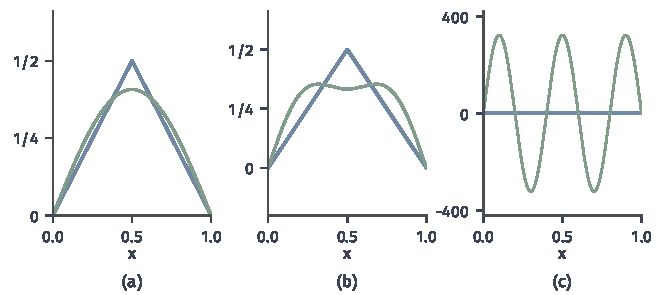
\includegraphics[width=112mm]{figures/06-differential-equations/02-partial-differential-equations/matplotlib/heat-inverse-recon/figure.pdf}
  \caption{截断重建，$T=0.05$，每个奇数模式的观测误差为$10^{-3}$。蓝线是真实的三角形，绿线是$u^{N}$。(a)$N=1$。(b)$N=3$。(c)$N=5$，注意纵轴范围。}
  \label{fig:heat-inverse-recon}
\end{BookInlineFigure}

\paragraph{Tikhonov滤波}
截断是硬开关。\term{Tikhonov正则化}（Tikhonov regularization）用平滑的滤波代替它。设$\sigma_k=\mathrm{e}^{-\lambda_kT}$，取$\alpha>0$，极小化
\[
 \lVert S(T)v-y\rVert_2^2+\alpha\lVert v\rVert_2^2 .
\]
这个问题按坐标分开，第$k$个坐标是一元二次函数，解为
\begin{equation}
 v_k=\frac{\sigma_k}{\sigma_k^2+\alpha}\,y_k .
 \label{eq:heat-tikhonov}
\end{equation}
增益$\sigma/(\sigma^2+\alpha)$在$\sigma=\sqrt\alpha$处最大，最大值是$1/(2\sqrt\alpha)$，所以噪声放大不超过这个数。$\sigma\gg\sqrt\alpha$的低频几乎按$1/\sigma$恢复，$\sigma\ll\sqrt\alpha$的高频被压到零。

取$\alpha=10^{-4}$，增益的上限是$50$。$T=0.05$时，$k=1,3,5$的增益分别是$1.64$、$49.3$、$0.044$，未正则化时是$1.64$、$84.9$、$2.3\times10^5$。图~\ref{fig:heat-inverse-tradeoff}(a)是不同噪声水平下总误差随$N$的变化，呈现先降后升的形状；图~\ref{fig:heat-inverse-tradeoff}(b)比较了三种增益。

\begin{BookInlineFigure}
  \centering
  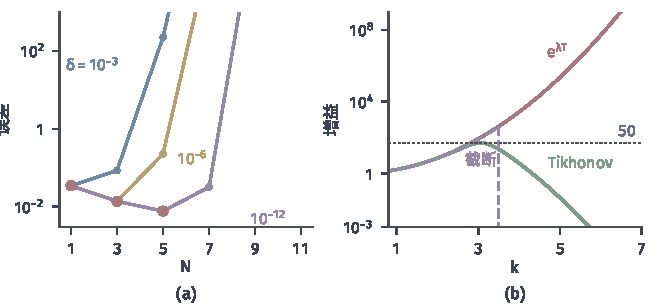
\includegraphics[width=112mm]{figures/06-differential-equations/02-partial-differential-equations/matplotlib/heat-inverse-tradeoff/figure.pdf}
  \caption{噪声与可恢复尺度。(a)三角形初值，$T=0.05$，每个奇数模式的观测误差$\delta=10^{-3},10^{-6},10^{-12}$时$L^2$总误差随$N$的变化，红点是最优的$N$。(b)作为连续变量$k$的增益：未正则化的$\mathrm{e}^{\lambda T}$（红）、截断（紫色虚线，示意取在$k=3.5$）、$\alpha=10^{-4}$的Tikhonov滤波（绿），点线是增益上限$50$。}
  \label{fig:heat-inverse-tradeoff}
\end{BookInlineFigure}

正则化并不能恢复已经丢失的信息，它只是诚实地放弃了高频，用先验（如初值的范数有界）换取稳定。正向过程越能抹平细节，反向过程就越难找回细节，这两者是同一个衰减因子的两面。
